\newpage
\subsection{Test}

Test bruges til at eftervise at vi har opnået vores krav. Test er en forsikring
på at vi har opfyldt de funktionelle samt nogle af de nonfunktionelle der er
blevet stillet i starten af projektet.

I dette projekt er det blevet anvendt unit tests til at teste små dele af
systemet. Når små dele af systemet af blevet test til fulde, kan de mindre dele
sættes sammen i systemets kontekst, her ville det være relevant at lave
integrationstest, hvor der testes på flere forskellige 'units'.

\subsubsection{Test af databasetransaktioner}%
\label{ssub:test_af_database_transaktioner}

I denne test vil tranaktioner med databasen blive testet. Hvis
persistenslaget skal fungere i en bredere kontekst, skal interaktionen med
databasen virke. Når denne kodeblok er blevet kaldt, da burde det være muligt at
hente denne person fra databasen.

\begin{lstlisting}
PersonManager.getInstance().addPerson(
    testPersonName,
    testPersonDesc,
    testPersonPhone,
    testPersonInfo,
    testPersonEmail
);
\end{lstlisting}

Vi fremsøger resultat i databasen og tjekker at det rigtige data er blevet
modtaget.

\begin{lstlisting}
ArrayList<IPerson> personResults 
    = PersonManager.getInstance().searchPerson(testPersonName);
for (IPerson person : personResults){
    if (person.getPhoneNumber().equals(testPersonPhone)){
        assertEquals(person.getName(), testPersonName);
        assertEquals(person.getDescription(), testPersonDesc);
        assertEquals(person.getPhoneNumber(), testPersonPhone);
        assertEquals(person.getPersonalInfo(), testPersonInfo);
        assertEquals(person.getPersonEmail(), testPersonEmail);
        personId = person.getCreditID();
        assertNotEquals(personId,0);
        try {
            database.deleteCredit(person);
            System.out.println("Removed person with creditID " + personId);
        } catch (Exception e){
            fail();
        }
    }
}
\end{lstlisting}

\begin{figure}
    \centering
    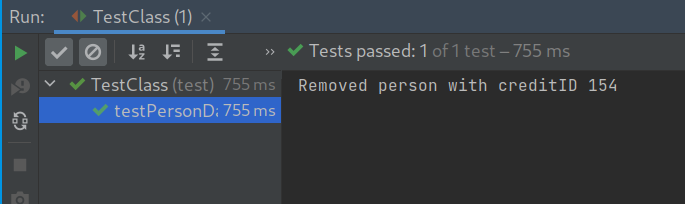
\includegraphics[width=0.5\textwidth]{images/test.png}
    \label{fig:test}
    \caption{Resultat af testen}
\end{figure}

\subsubsection{Andre test}%
\label{ssub:andre_test}

Det ville selvfølgelig være relevant at teste om de forskellige funktioner der
indgår vores brugsmønsterrealiseringer lever op til de kontrakter der tildelt
dem. Fx om søgefunktionen faktisk returnerer de korrekte værdier ved forskellige
søgestrenge. Som beskrevet i \cite[s.
236]{book:sommeville_software_engineering}, skal der testes på forskellige
partitioner af søgestrenge. 
